%% \documentclass[9pt,handout]{beamer}

\documentclass[9pt,aspectratio=1610]{beamer}
\usepackage{color,fancybox,alltt,graphicx}

\usepackage{pgf,pgfarrows,pgfnodes,pgfautomata,pgfheaps,pgfshade}

\usepackage[latin1]{inputenc}
\usepackage{colortbl}
\usepackage[english]{babel}
\usepackage{multimedia}
\usepackage{amssymb,amsmath}
\usepackage{ragged2e}
\usepackage{animate}
\usepackage{listings}

\newif\ifpdf
\ifx\pdfoutput\undefined
\pdffalse % we are not running PDFLaTeX
\else
\pdfoutput=1 % we are running PDFLaTeX
\pdftrue
\fi

\mode<article>{ \usepackage{fullpage}  \usepackage{pgf}  \usepackage{hyperref} }


\mode<presentation>{
  \usetheme{XAFS}
  \setbeamercovered{transparent}
}

\usepackage{amsmath}
\usepackage{tikz}

\usepackage[customcolors,shade]{hf-tikz}

\usetikzlibrary{calc}

% put color to \boxed math command
\newcommand*{\cmboxcolor}{orange}
\makeatletter
\newcommand{\cmbox}[1]{\textcolor{\cmboxcolor}{%
 \makeatother
\tikz[baseline={([yshift=-1ex]current bounding box.center)}] \node [rectangle, minimum width=1ex,rounded corners,draw] {\normalcolor\m@th$\displaystyle#1$};}}



\usepackage[latin1]{inputenc}
\usepackage[english]{babel}
\setbeamertemplate{navigation symbols}{}

\setlength{\fboxrule}{1pt}


\newcommand{\vmm}{{\vspace{2mm}}}
\newcommand{\hmm}{{\hspace{1mm}}}
\newcommand{\Justify}{\justify\vspace{-\baselineskip}}

\newcommand{\Program}[1]{\scshape{#1}}
\newcommand{\atoms}{{\Program{atoms}}}
\newcommand{\feffit}{{\Program{feffit}}}
\newcommand{\ifeffit}{{\Program{ifeffit}}}
\newcommand{\larch}{{\Program{larch}}}
\newcommand{\xasviewer}{{\Program{XAS Viewer}}}

\newcommand{\ease}{{\Program{EASE}}}
\newcommand{\autobk}{{\Program{autobk}}}
\newcommand{\ffchi}{{\Program{ff2chi}}}
\newcommand{\diffkk}{{\Program{diffkk}}}
\newcommand{\sixpack}{{\Program{sixpack}}}
\newcommand{\hephaestus}{{\Program{hephaestus}}}
\newcommand{\athena}{{\Program{athena}}}
\newcommand{\artemis}{{\Program{artemis}}}
\newcommand{\feff}{{\Program{feff}}}
\newcommand{\mxan}{{\Program{mxan}}}
\newcommand{\fdmnes}{{\Program{fdmnes}}}
\newcommand{\gnuplot}{{\Program{gnuplot}}}

\newcommand{\file}[1]{{{\slshape\ttfamily{#1}}}}
\newcommand{\feffndat}{\file{feffnnnn.dat}}
\newcommand{\feffbin}{\file{feff.bin}}


\newcommand{\bmu}{{\mu}}
\newcommand{\bepsilon}{{\epsilon}}
\newcommand{\bDelta}{{\Delta}}
\newcommand{\bOmega}{{\Omega}}
\newcommand{\bdelta}{{\delta}}
\newcommand{\bsigma}{{\sigma}}
\newcommand{\bln}{{\ln}}
\newcommand{\bsum}{{\sum}}
\newcommand{\bsim}{{\sim}}
\newcommand{\bsin}{{\sin}}
\newcommand{\bexp}{{\exp}}
\newcommand{\bint}{{\int}}
\newcommand{\bpsi}{{\psi}}
\newcommand{\bpropto}{{\propto}}
\newcommand{\bapprox}{{\approx}}
\newcommand{\bchi}{{\chi}}
\newcommand{\brho}{{\rho}}
\newcommand{\bpi}{{\pi}}
\newcommand{\balpha}{{\alpha}}
\newcommand{\bbeta}{{\beta}}
\newcommand{\blambda}{{\lambda}}
\newcommand{\blesssim}{{\lesssim}}
\newcommand{\brightarrow}{{\rightarrow}}
\newcommand{\bAA}{{\rm\AA}}
\newcommand{\mbf}[1]{{\ensuremath{\mathbf\mathit{#1}}}}

\newcommand{\chie}{{\ensuremath{\chi(E)}}}
\newcommand{\chik}{{\ensuremath{\chi(k)}}}
\newcommand{\chir}{{\ensuremath{\chi(R)}}}
\newcommand{\mue}{{\ensuremath{\mu(E)}}}
\newcommand{\bkg}{{\ensuremath{\mu_0(E)}}}

\definecolor{lightyellow}{rgb}{1.0,1.0,0.8}
\definecolor{lightyellow2}{rgb}{1.0,1.0,0.97}
\definecolor{golden}{rgb}{0.75,0.75,0.37}
\definecolor{lightpink}{rgb}{1.0,0.9,0.9}
\definecolor{nearwhite}{rgb}{0.95,0.94,0.94}
\definecolor{verywhite}{rgb}{0.99,0.99,0.99}
\definecolor{white}{rgb}{1.0,1.0,1.0}
\definecolor{DarkBlue}{rgb}{0,0,0.3}
\definecolor{BrightBlue}{rgb}{0,0,0.7}
\definecolor{DarkRed}{rgb}{0.65,0,0}
\definecolor{BrightRed}{rgb}{0.8,0,0}
\definecolor{RRed}{rgb}{0.95,0,0}
\definecolor{BlueGrey}{rgb}{0.2,0.1,0.1}

\definecolor{VBlue}{rgb}{0,0,0.9}
\definecolor{BrightGreen}{rgb}{0,0.6,0.0}
\definecolor{DarkGreen}{rgb}{0,0.3,0}


\newcommand{\Color}[2]{{\textcolor{#1}{#2}}}
\newcommand{\Red}[1]{{\Color{BrightRed}{#1}}}
\newcommand{\RRed}[1]{{\Color{RRed}{#1}}}
\newcommand{\DarkRed}[1]{{\Color{DarkRed}{#1}}}
\newcommand{\Blue}[1]{{\Color{BrightBlue}{#1}}}
\newcommand{\BrightBlue}[1]{{\Color{BrightBlue}{#1}}}
\newcommand{\Black}[1]{{\Color{black}{#1}}}
\newcommand{\RedM}[1]{{\Color{red}{\mbf{#1}}}}
\newcommand{\BlueM}[1]{{\Color{blue}{\mbf{#1}}}}
\newcommand{\BlackM}[1]{{\Color{black}{\mbf{#1}}}}


\newcommand{\DarkGreen}[1]{{\Color{DarkGreen}{#1}}}
\newcommand{\DarkBlue}[1]{{\Color{DarkBlue}{#1}}}


\newcommand{\RedEmph}[1]{{\Color{BrightRed}{\emph{#1}}}}
\newcommand{\RedSl}[1]{{\Color{BrightRed}{\slshape{#1}}}}
\newcommand{\BlueSl}[1]{{\Color{BrightBlue}{\slshape{#1}}}}
\newcommand{\BlueEmph}[1]{{\Color{BrightBlue}{\emph{#1}}}}


\newcommand{\LString}[1]{{\Color{BrightGreen}{{#1}}}}
\newcommand{\LKeyword}[1]{{\Color{DarkRed}{{#1}}}}
\newcommand{\LFunc}[1]{{\Color{VBlue}{{#1}}}}
\newcommand{\LComment}[1]{{\Color{BrightRed}{{#1}}}}


\newcommand{\pthpar}[1]{{\ensuremath{{\tt{\Blue{#1}}}}}}

\newcommand{\feffc}[1]{{{\ensuremath{{\Red{#1}}}}}}
\newcommand{\reff}{{{\feffc{R_{\rm eff}}}}}
\newcommand{\twothirds}{{{\textstyle{2 \over 3}}}}
\newcommand{\fourthirds}{{{\textstyle{2 \over 3}}}}
\newcommand{\masse}{{({{2m_e} / {\hbar^2}})}}

\newcommand{\highlightbox}[1]{{ \fcolorbox{black}{lightyellow}{#1}}}

\newenvironment{VerbSBox}[1]%
{\VerbatimEnvironment\begin{Sbox}%
\begin{minipage}{#1}\begin{alltt}}%
{\end{alltt}\end{minipage}\end{Sbox}\setlength{\fboxsep}{2mm}{%
\begin{flushright}\shadowbox{\TheSbox}\end{flushright}}}
%%

\newenvironment{VerbSSBox}[1]%
{\VerbatimEnvironment\begin{Sbox}%
\begin{minipage}{#1}\begin{alltt}}%
{\end{alltt}\end{minipage}\end{Sbox}\setlength{\fboxsep}{2mm}{%
\begin{center}\shadowbox{\TheSbox}\end{center}}}
%%

% \newenvironment{VerbBox}[1]%
% {\VerbatimEnvironment\begin{Sbox}%
% \begin{minipage}{#1}\begin{alltt}}%
% {\end{alltt}\end{minipage}\end{Sbox}\setlength{\fboxsep}{2mm}{%
% \shadowbox{\TheSbox}
% %%

\newenvironment{CodeBlock}[2]%
{\VerbatimEnvironment\begin{minipage}{#1}\begin{block}{\small{#2}}\begin{semiverbatim}\tiny}%
{\end{semiverbatim}\end{block}\end{minipage}}%%

\definecolor{DeepGrey}{rgb}{0.15,0.05,0.05}
\newcommand{\GreyLine}{{\color{DeepGrey}{\rule{\linewidth}{1.00pt}}}}

\newcommand{\STitle}[1]{{\hspace{2mm}{\bfseries\sl\Large%
      \BrightBlue{#1}}}\hfill\par%
  \vspace{-3.5mm}\GreyLine\vspace{-0.1mm}}

\newenvironment{ListingBlock}[2]%
{\begin{minipage}{#1}\begin{block}{\small{#2}}\begin{lstlisting}}
{\end{lstlisting}\end{block}\end{minipage}}%%

\newenvironment{figblock}[3]%
{\begin{minipage}{#1}\begin{exampleblock}{#2}{\wgraph{#1}{#3}}}%
{\end{exampleblock}\end{minipage}}%

\newenvironment{MFrame}[1]%%
{\subsection{#1}\begin{frame}\frametitle{#1}}%
{\end{frame}}%

\newenvironment{Boxedminipage}%
    {\begin{Sbox}\begin{minipage}}%
    {\end{minipage}\end{Sbox}\shadowbox{\TheSbox}}


\setbeamercolor{postit}{fg=black,bg=lightyellow}

\newenvironment{postitbox}[1]%%
{\begin{center}\begin{minipage}{#1}\begin{beamercolorbox}[shadow=true,rounded=true]{postit}}%
{\end{beamercolorbox}\end{minipage}\end{center}}%


\newenvironment{postitboxC}%%
{\begin{center}\begin{beamercolorbox}[center,shadow=true,rounded=true]{postit}}%
{\end{beamercolorbox}\end{center}}%

\newcommand{\entrylabel}[1]{ {\Blue{#1:}}}
%%\newcommand{\entrylabel}[1]{{\parbox[b]{10mm}{%
%%      \makebox[10mm][l]{{\Red{#1:}}}\\}}}

\newenvironment{entry}
{\begin{list}{}{\renewcommand{\makelabel}{\entrylabel}%
      \setlength{\labelwidth}{7mm}
      \setlength{\leftmargin}{6mm}}}{\end{list}}

\newcommand{\redlabel}[1]{ {\Color{DarkRed}{#1}}}
\newenvironment{redlist}[1]{\begin{list}{}{\renewcommand{\makelabel}{\redlabel}%
      \setlength{\leftmargin}{#1}}}{\end{list}}


\newcommand{\bluelabel}[1]{ {\Color{BrightBlue}{#1}}}
\newenvironment{bluelist}[1]{\begin{list}{}{\renewcommand{\makelabel}{\bluelabel}%
      \setlength{\leftmargin}{#1}}}{\end{list}}

\newcommand{\xbluelabel}[1]{{\Color{BrightBlue}{#1\hspace{2mm}}}}
\newenvironment{xbluelist}[1]{\begin{list}{}{\renewcommand{\makelabel}{\xbluelabel}%
      \setlength{\leftmargin}{#1}}}{\end{list}}

\newenvironment{cenpage}[1]%%  centered minipage
{\begin{center}\begin{minipage}{#1}}%
    {\end{minipage}\end{center}}%%

\newenvironment{slide}[1]%%  begin named slide
{\begin{frame}\frametitle{#1}}%
{\end{frame}}%%

\newenvironment{fslide}[1]%%  begin named slide
{\subsection{#1}\begin{frame}[fragile]\frametitle{#1}}%
{\end{frame}}%%


\newcommand{\xdgraph}[2]{{%
        \ifpdf  \includegraphics[width={#1}]{figs/#2.png}%
        \else   \includegraphics[width={#1}]{figs/#2.eps}\fi}}

\newcommand{\rgraph}[2]{\includegraphics[width={#1}]{figs/rimg/#2}}
\newcommand{\wgraph}[2]{\includegraphics[width={#1}]{figs/#2.png}}
\newcommand{\hgraph}[2]{\includegraphics[height={#1}]{figs/#2.png}}
\newcommand{\wpdf}[2]{\includegraphics[width={#1}]{#2.pdf}}

\newcommand{\webpage}[1]{{{\Blue{{#1}}}}}

%% \pgfdeclareimage[interpolate=true,width=45mm]{xafscartoon}{figs/xafsabsorb}
%% \pgfdeclareimage[interpolate=true,width=50mm]{xafsxanes}{figs/xafsxanes}
%% \pgfdeclareimage[interpolate=true,width=50mm]{feff}{figs/scattamp}
%% \pgfdeclareimage[interpolate=true,width=55mm]{tdlplot}{figs/tdlplot}

%% \pgfdeclareimage[interpolate=true,width=15mm]{ravel}{figs/RavelHead}
%% \pgfdeclareimage[interpolate=true,width=15mm]{calvin}{figs/CalvinHead}
%% \pgfdeclareimage[interpolate=true,width=15mm]{frenkel}{figs/FrenkelHead}
%% \pgfdeclareimage[interpolate=true,width=15mm]{haskel}{figs/HaskelHead}
%% \pgfdeclareimage[interpolate=true,width=15mm]{jox}{figs/JoxHead}
%% \pgfdeclareimage[interpolate=true,width=15mm]{newville}{figs/NewvilleHead}
%% \pgfdeclareimage[interpolate=true,width=15mm]{kelly}{figs/KellyHead}

%% \pgfdeclareimage[interpolate=true,width=15mm]{rehr}{figs/RehrHead}
%% \pgfdeclareimage[interpolate=true,width=15mm]{fons}{figs/FonsHead}
%% \pgfdeclareimage[interpolate=true,width=15mm]{webb}{figs/WebbHead}
%% \pgfdeclareimage[interpolate=true,width=15mm]{glover}{figs/GloverHead}
%% \pgfdeclareimage[interpolate=true,width=15mm]{trainor}{figs/TrainorHead}

%% \pgfdeclareimage[interpolate=true,width=85mm]{APS2005_Photo}{figs/APS2005_Photo}

%% \pgfdeclareimage[interpolate=true,width=68mm]{EASE}{figs/EASE}



\begin{document}

\title[Virtual XAFS School]{X-ray Absorption Fine-Structure Spectroscopy: Theory}
\author[M Newville]{Matthew Newville}
\date{July-2021}

\institute[Univ of Chicago]{Center for Advanced Radiation Sources\\
  The University of Chicago}


\begin{frame} \titlepage

  \vmm

  \begin{center}
    Fundamentals of X-ray Absorption Fine-Structure
  \end{center}
  
  \vmm

  \begin{cenpage}{60mm}
    Virtual XAFS School at Illinois Institute of Technology and Advanced
  Photon Source
\end{cenpage}
\end{frame}


\section{X-ray Absorption Spectroscopy}

 %% Slide
\subsection{What is XAS}

\begin{frame} \frametitle{X-ray Absorption Spectroscopy:  XAS, XAFS,  EXAFS and XANES.}

  \begin{cenpage}{125mm}

    X-ray Absorption Spectroscopy ({\Blue{XAS}}) is the modulation of
    the X-ray absorption coefficient at energies at and above an X-ray
    absorption edge.

    \vmm
    \begin{center}
      \begin{tabular}{ll}
        {\Blue{XAFS}} &  X-ray Absorption Fine-Structure Spectroscopy  (= XAS) \\
        {\Blue{XANES}} & X-ray Absorption Near-Edge Spectroscopy\\
        {\Blue{EXAFS}} & Extended X-ray Absorption Fine-Structure \\
      \end{tabular}
    \end{center}
    \vspace{1mm}

    These contain information about an element's chemical state (XANES) and
    local atomic environment (EXAFS).

    \end{cenpage}


    \begin{columns}[T]
      \begin{column}{62mm}
        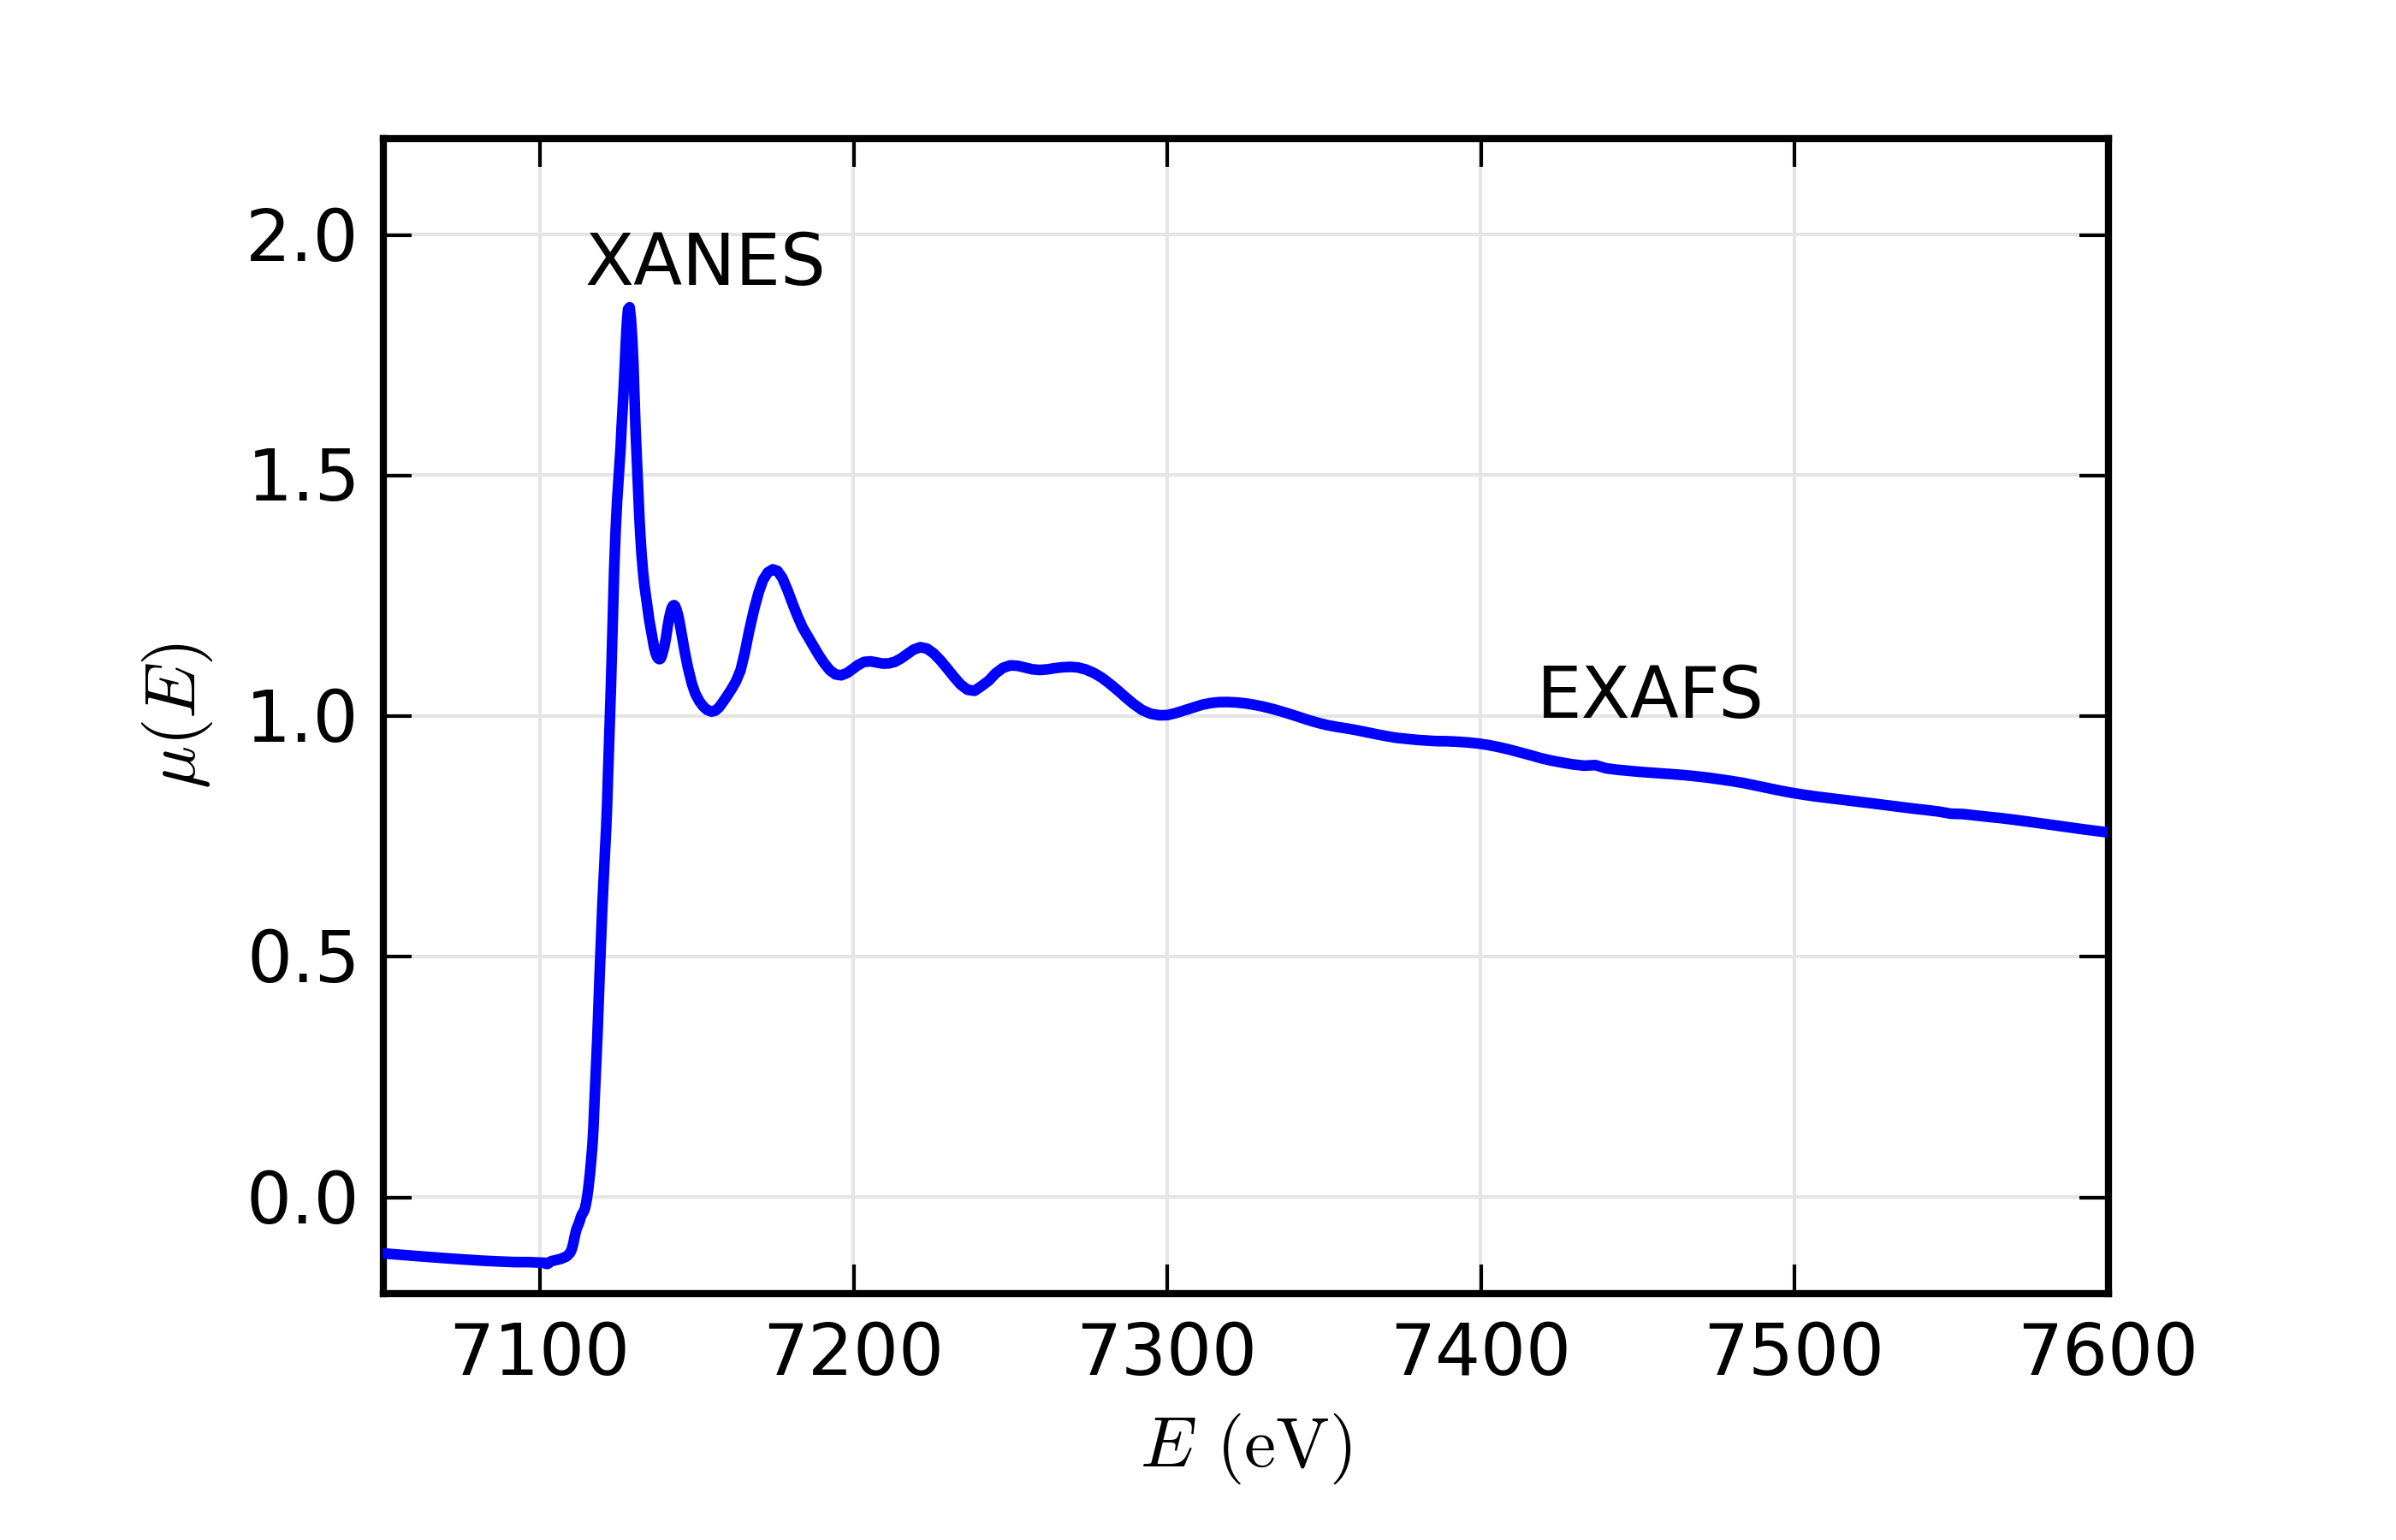
\includegraphics[width=58mm]{figs/rimg/mu_xanes_exafs}

        {\hspace{10mm} Fe {\slshape{K}}-edge XAFS for FeO}
      \end{column}
      \begin{column}{65mm}
        {\RedEmph{Main XAS Characteristics}}:
        \begin{itemize}
        \item local atomic coordination
        \item valence, oxidation state
        \item applies to any element ($Z > 2$) .
        \item works at low concentrations (ppm, $\mu$M)
        \item minimal sample requirements.
        \item independent of crystal  structure, isotope.
        \end{itemize}
      \end{column}
    \end{columns}

\vfill
\end{frame}

 
\begin{slide}{XANES:  X-ray Absorption Near-Edge Spectroscopy}
\begin{cenpage}{120mm}
 Within $\sim$100eV of the absorption edge, the X-ray Absorption Spectra is
 highly sensitive to the chemical state and formal valence of absorbing element:
\end{cenpage}

\begin{cenpage}{150mm}
  \vmm
  \begin{columns}
    \begin{column}{48mm}
      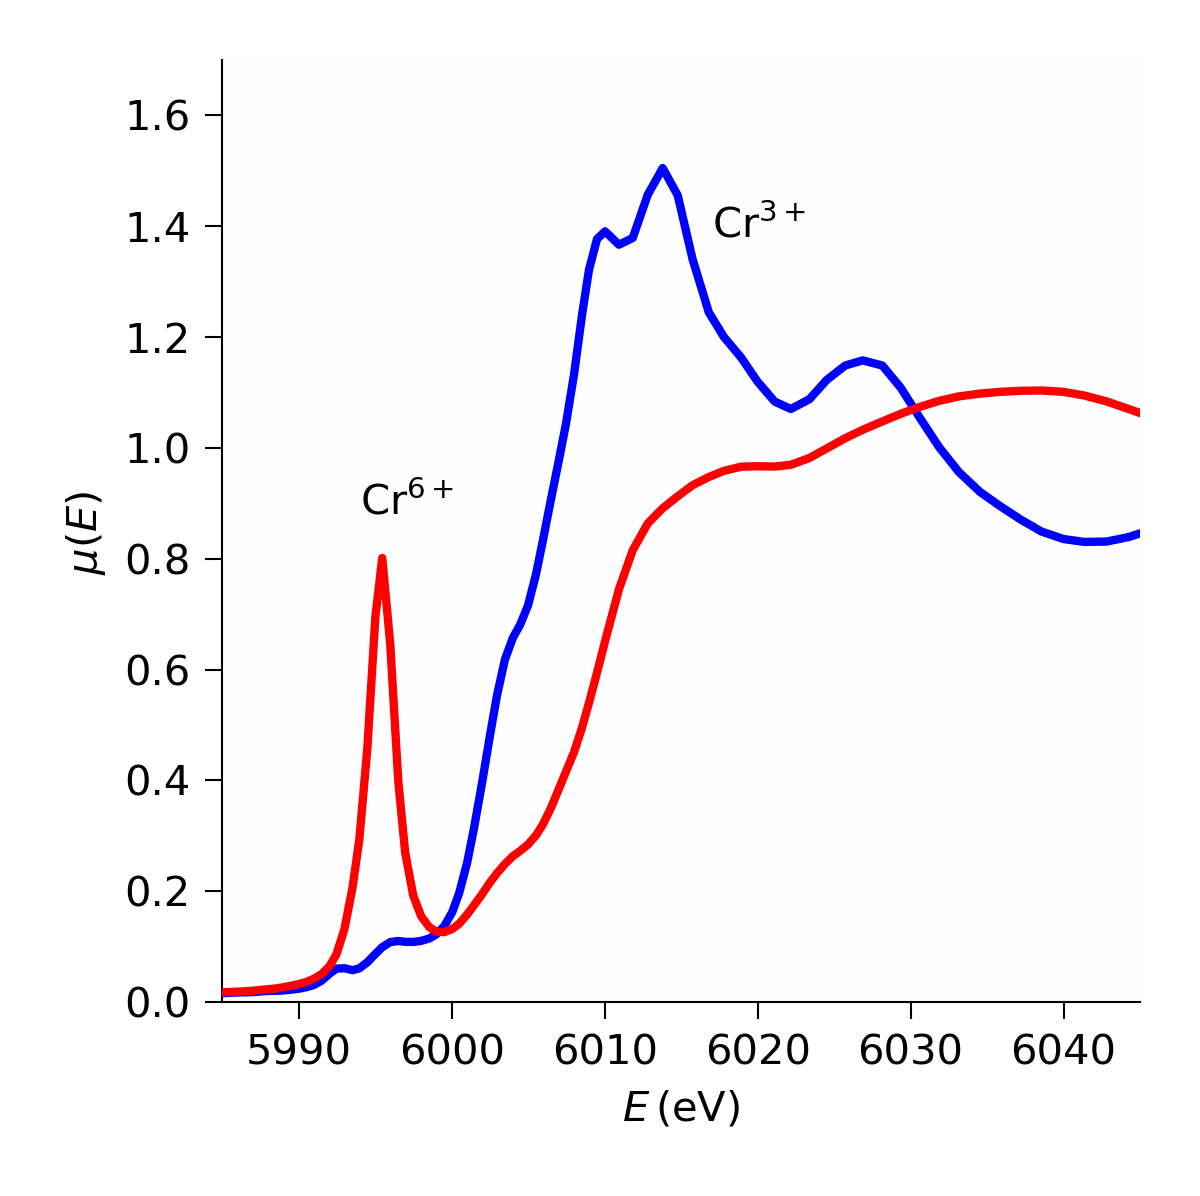
\includegraphics[width=48mm]{figs/xanes/cr}

      \vmm
      \hspace{5mm}  $\rm Cr^{3+}$ and $\rm Cr^{6+}$
    \end{column}
    \begin{column}{48mm}    
      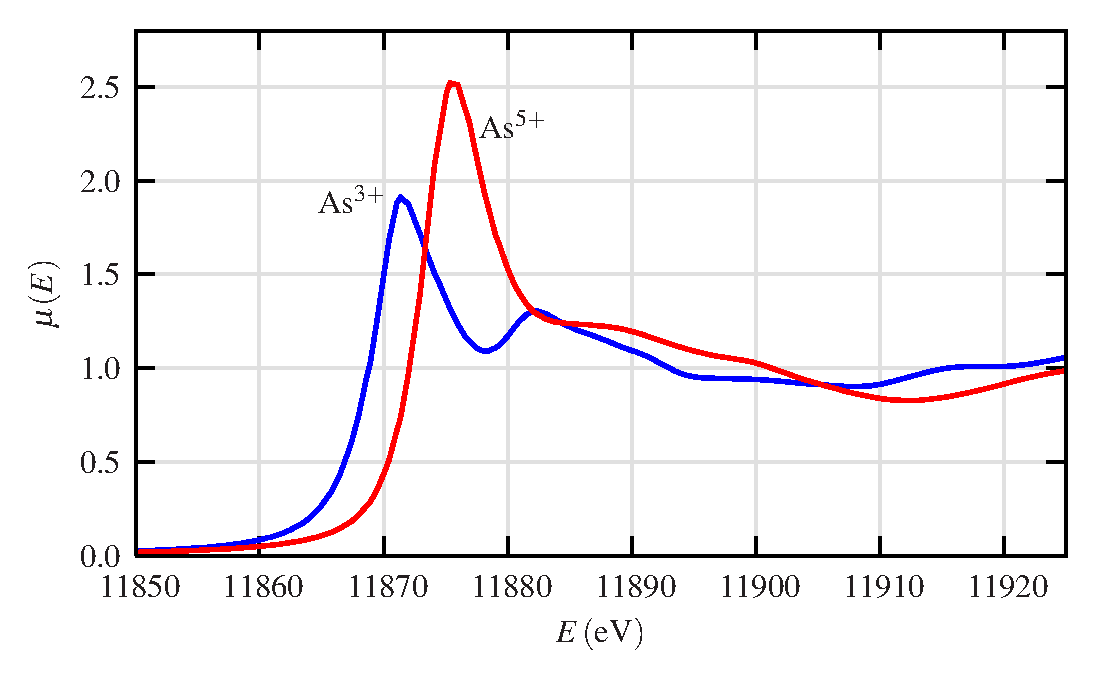
\includegraphics[width=48mm]{figs/xanes/as}
      
      \vmm
      \hspace{5mm}    $\rm As^{3+}$ and $\rm As^{5+}$
    \end{column}

    \begin{column}{48mm}
     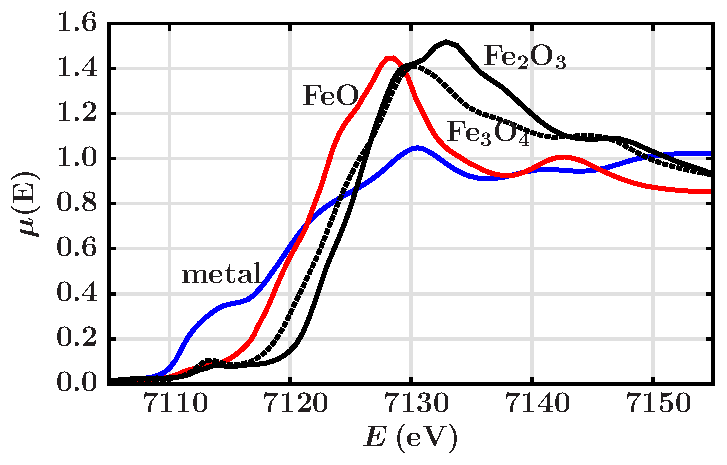
\includegraphics[width=48mm]{figs/xanes/fe_oxides}
      \hspace{5mm}    Fe metal and oxides.
    \end{column}
  \end{columns}

  \vmm
  
    The oxidation state and local atomic coordination environment strongly
    affect the lowest unfilled electronic levels of an absorbing atom.

    \vmm
    \begin{center}
      
    \begin{postitbox}{105mm}
        {\BlueEmph{what are the unoccupied electronic states
            that the photo-electron can fill?}}
    \end{postitbox}
  \end{center}

  \end{cenpage}

\vfill
\end{slide}


 
\begin{slide}{EXAFS: Extended X-ray Absorption Fine Structure}


\begin{cenpage}{108mm}
  Even far above the edge, there are oscillations in $\mu(E)$ that are
  sensitive to the positions and types of atoms neighboring the absorbing
  atom.
\vmm

 We define the EXAFS as:

  \[
  \mu(E) =   \mu_0(E) [1 + \chi(E)]  \hspace{15mm} \chi(E) =   \frac{ {\mu(E) - \mu_0(E)}}{\Delta \mu_0(E_0)}
  \]

  We subtract off a smooth {\BlueEmph{``bare atom'' background}}
  $\mu_0(E)$, and divide by the {\BlueEmph{``edge step''}}
  $\Delta \mu_0(E_0)$ to get $\chi$, the EXAFS oscillations:

\end{cenpage}

\begin{tabular}{ll}
  \onslide+<1->
  \begin{minipage}{55mm}
    \rgraph{55mm}{mu_with_mu0}
  \end{minipage}
  &
  \onslide+<1->
  \begin{minipage}{55mm}
    \rgraph{55mm}{chie}
  \end{minipage} \\
%%   \noalign{\smallskip}\\
  \onslide+<1->
  \hspace{3mm} $\mu(E)$ and $\mu_0(E)$ for FeO
  &
  \onslide+<1->
  \hspace{3mm} $\chi(E)$ for FeO, with $E_0$ = 7122 eV.
\end{tabular}

\vfill
\end{slide}

 
\begin{slide}{EXAFS: $\chi(k)$ and XAFS Fourier Transforms}

  \begin{cenpage}{120mm}

    EXAFS is an {\RedEmph{interference effect}}, using the wave-nature of
    the photo-electron.  We express the XAFS in terms of
    {\RedEmph{photo-electron wavenumber}}, ${k}$:

    \[  k= \sqrt{  \frac{2m(E-E_0)}{ {\hbar}^2} } \]

We'll also then use Fourier Transforms to convert from $k$ to  $R$.
\vmm



   \begin{columns}[T]
     \begin{column}{65mm}
       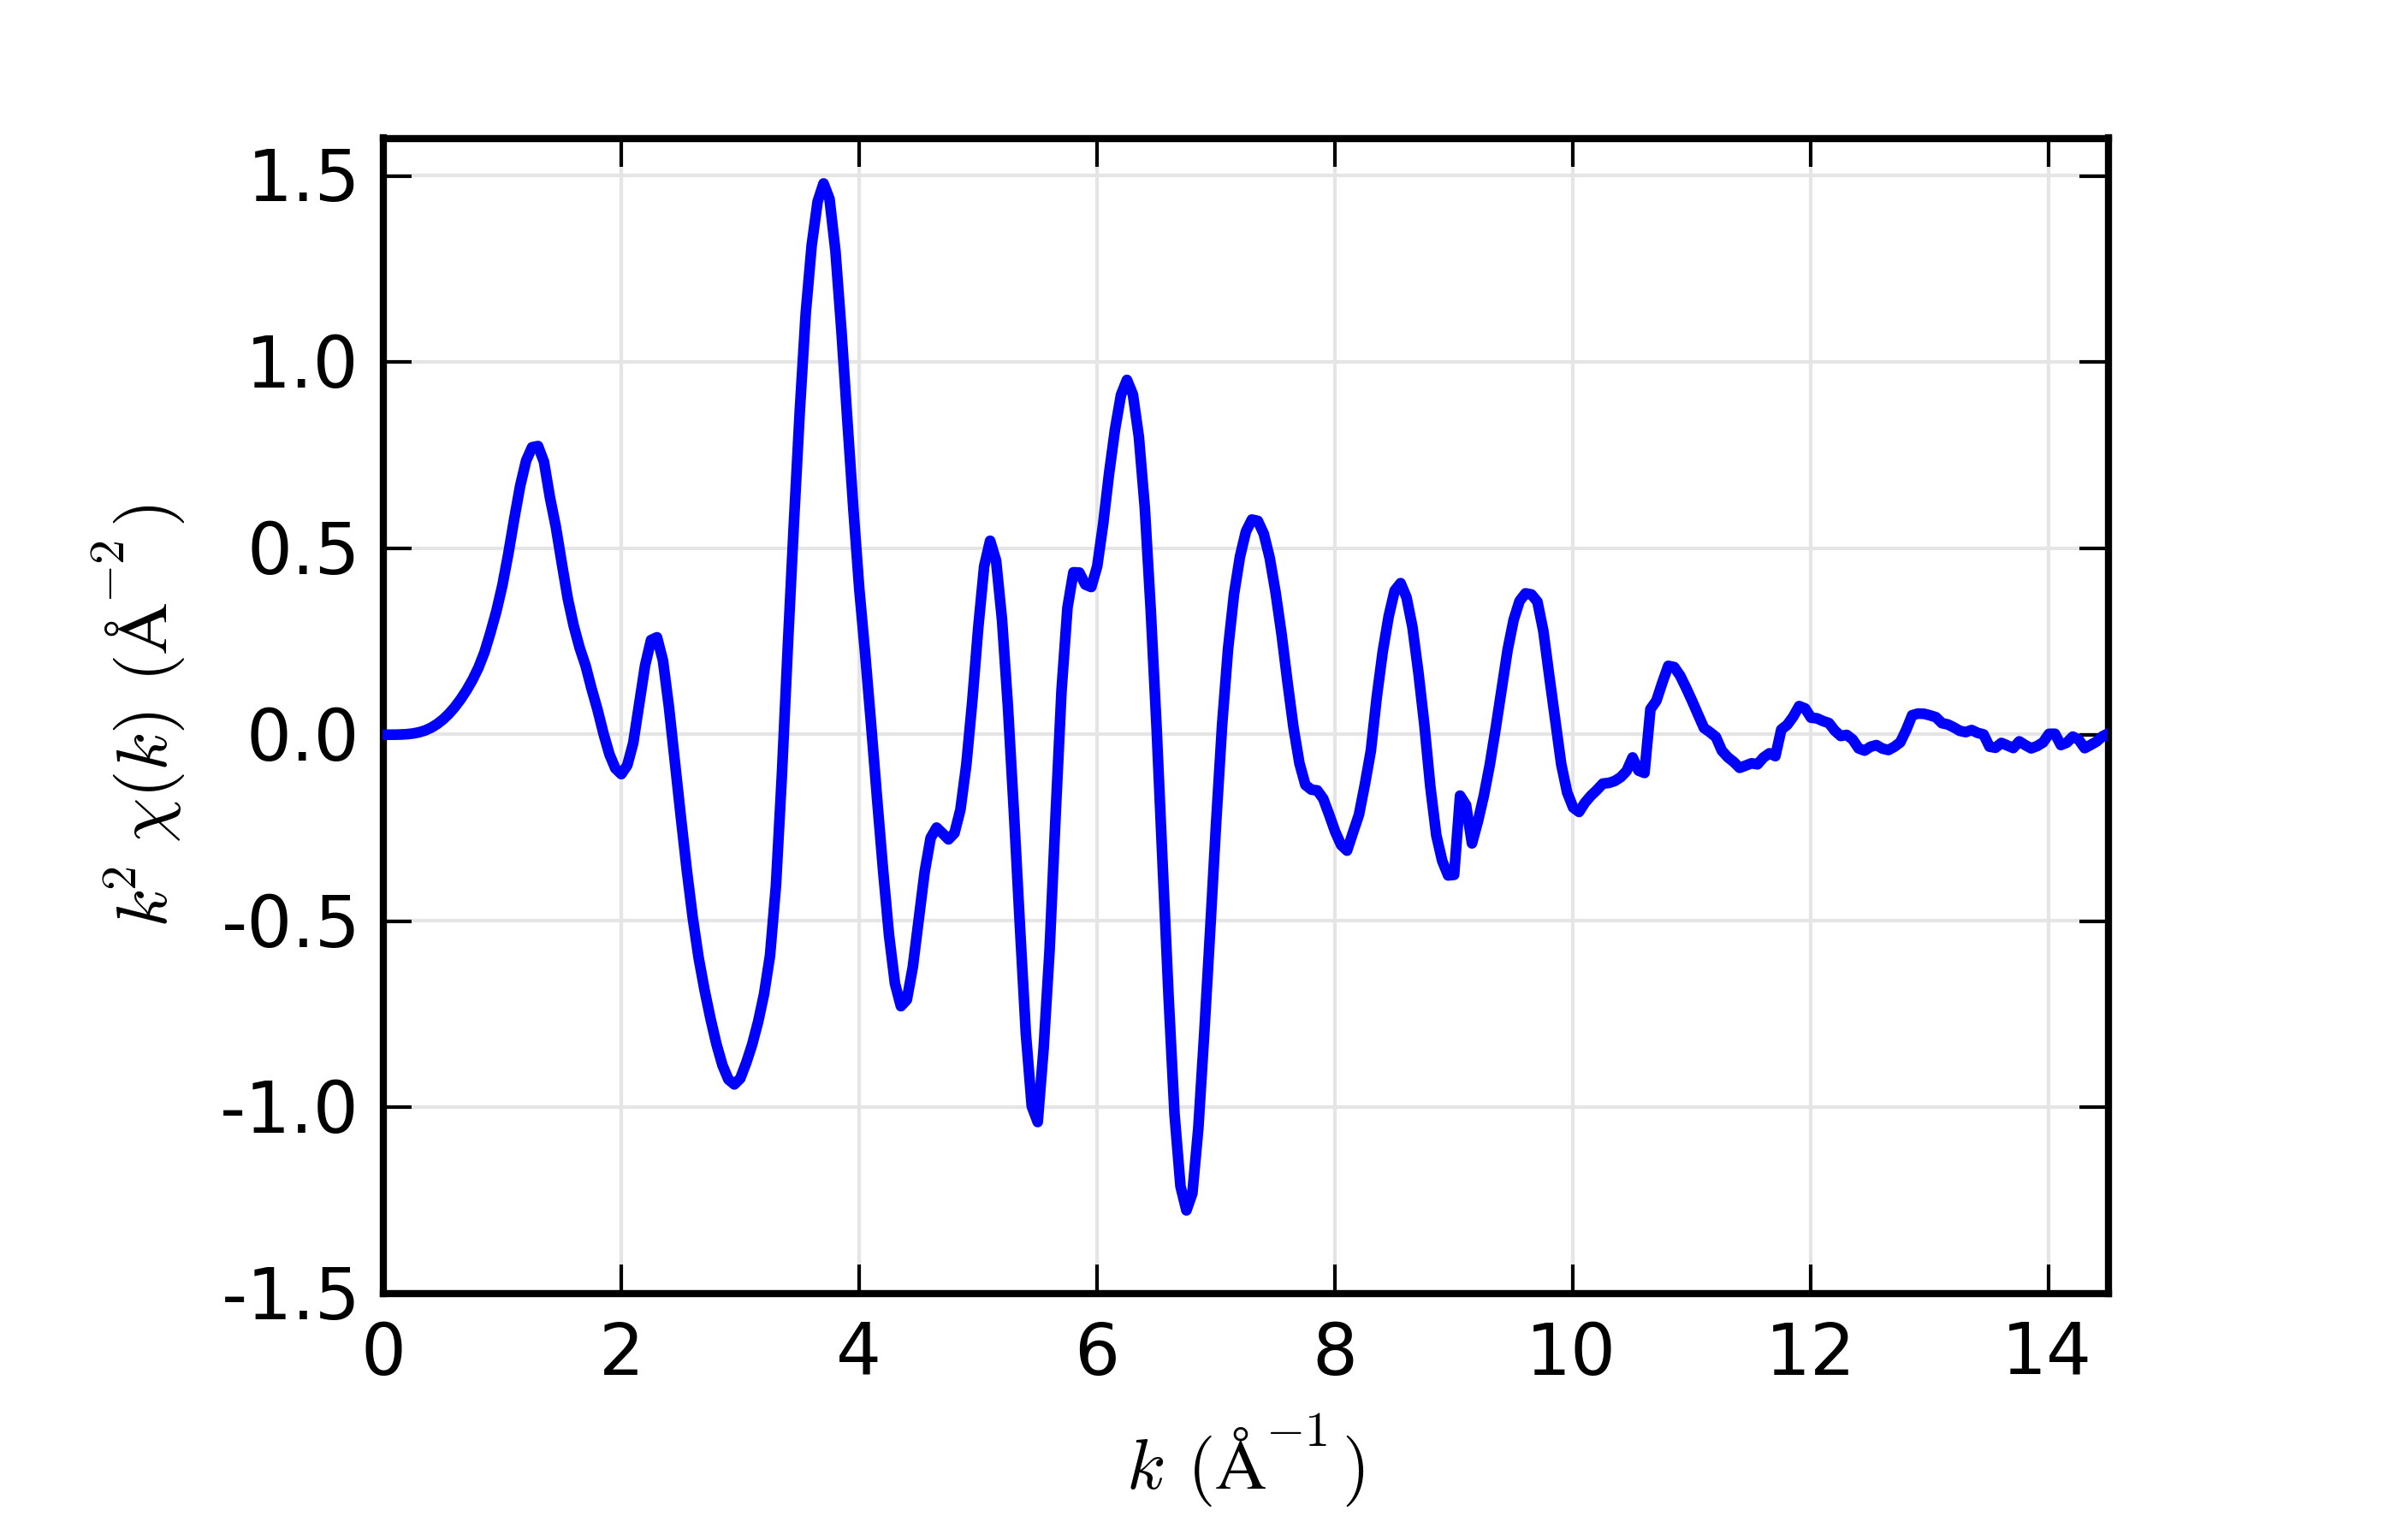
\includegraphics[width=58mm]{figs/rimg/feo_chik}
       \hspace{10mm} $k^2\chi(k)$ for FeO       
     \end{column}
     \begin{column}{65mm}
       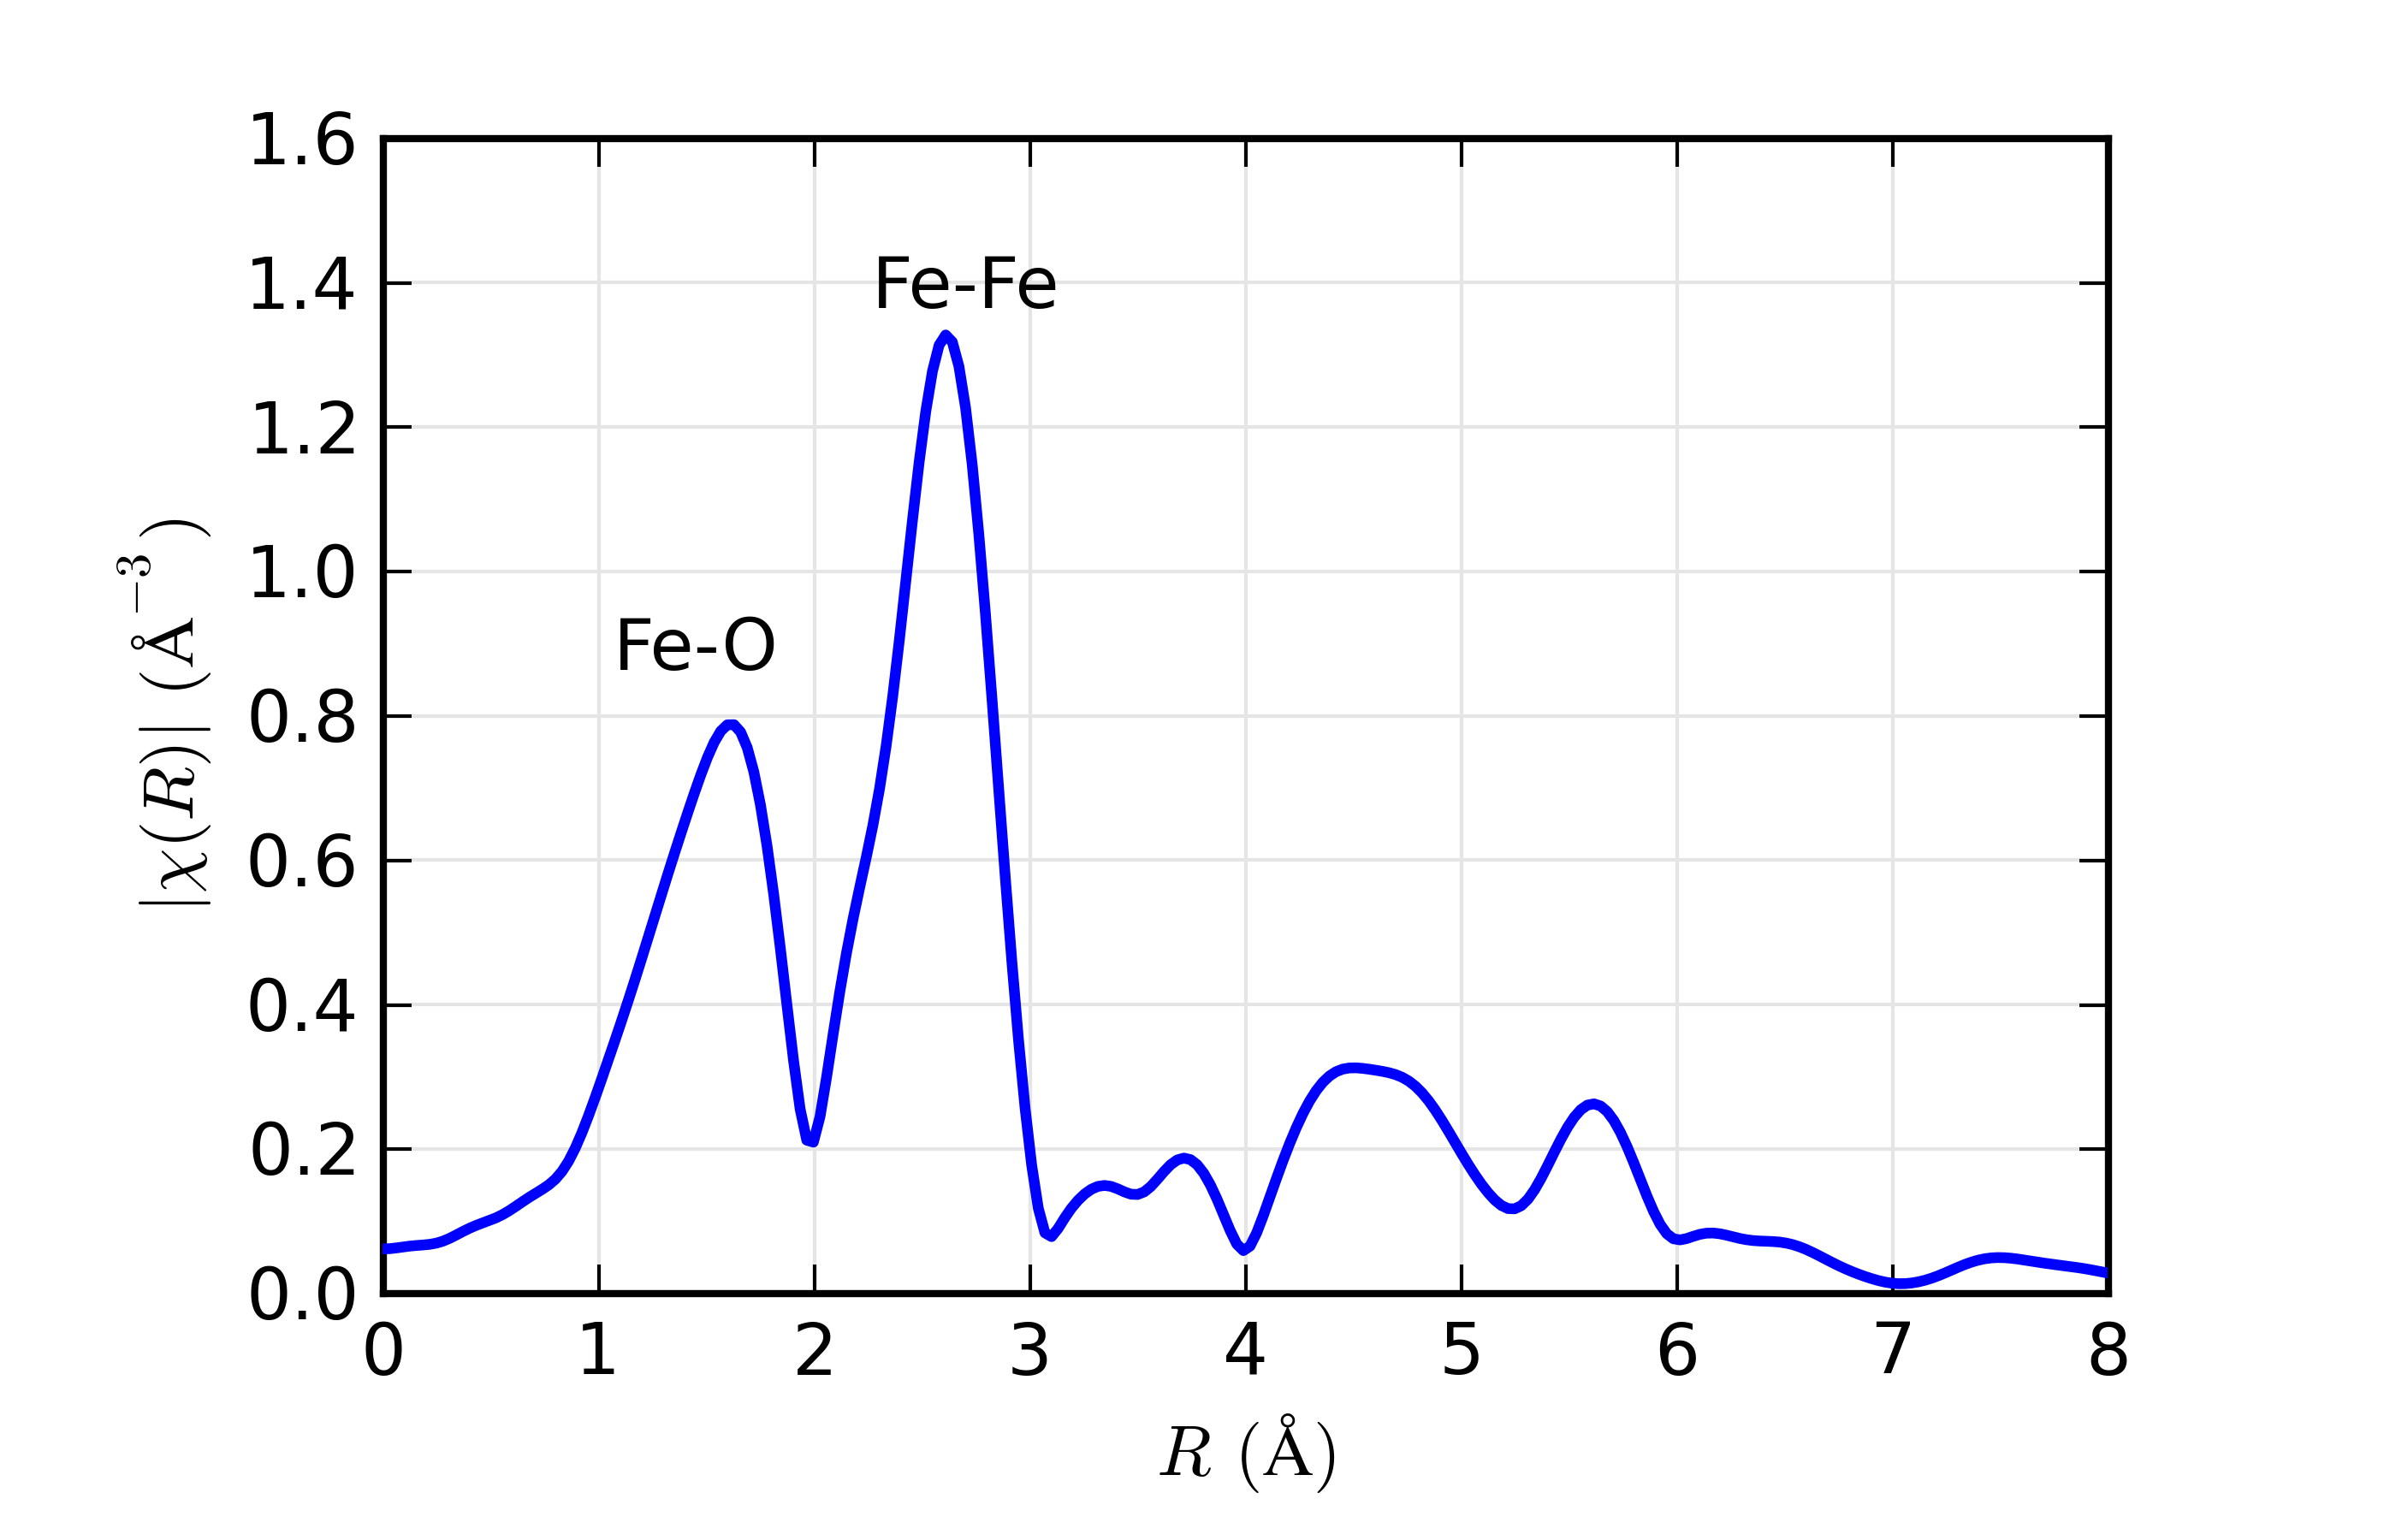
\includegraphics[width=58mm]{figs/rimg/feo_chir}
       \hspace{10mm}   Fourier Transform $|\chi(R)|$ for FeO. \par
       Similar to a Pair Distribution Function.
       
     \end{column}     
   \end{columns}


\end{cenpage}

\end{slide}

 \begin{slide}{The EXAFS Equation}


  \begin{cenpage}{120mm}

    To model the EXAFS, we use the {\BlueEmph{EXAFS Equation}}:
  \vspace{-1mm}

  \begin{center}
    \[ \chi(k) = \sum_j {\frac{{\Blue{N_j}} {\Red{f_j(k)}}
        e^{-2{\Blue{R_j}}/{\Red{\lambda(k)}}}
        e^{-2k^2{\Blue{\sigma_j^2}}}}{k{\Blue{R_j}}^2}
      {\sin[{2k{\Blue{R_j}} + {\Red{\delta_j(k)}}] }}} \]
  \end{center}

  \vmm

  where $\Red{f(k)}$ and $\Red{\delta(k)}$ are
  {\RedEmph{photo-electron scattering properties}} of the neighboring
  atom [and $ \Red{\lambda(k)} $ is the photo-electron mean-free-path].

  \vmm
  If we know these properties, we can determine:
  \onslide+<2->
    \begin{description}
      \settowidth{\labelwidth}{15mm}
      \setlength{\itemindent}{15mm}
      \setlength{\leftmargin}{15mm}
    \item[$R$] distance to neighboring atom.
    \item[$N$] coordination number of neighboring atom.
    \item[$\sigma^2$] mean-square disorder of neighbor distance.
    \end{description}

  \vmm
  \onslide+<3>
  ${\Red{f(k)}}$ and ${\Red{\delta(k)}}$ depend on atomic number
  {\BlueEmph{Z}} of the scattering atom, so we can also determine the
  species of the neighboring atom.


\end{cenpage}

\end{slide}



 \section{X-ray Absorption Theory}

 \begin{slide}{XAFS Theory}
    \vspace{3mm}
    \begin{center}
      {\Huge\BlueEmph{Development of the EXAFS Equation}}
    \end{center}
  \vfill
\end{slide}

  \begin{slide}{X-ray Absorption by a Free Atom}

  \Justify An atom absorbs an x-ray (energy $E$), destroying a core electron (energy
  ${E_0}$) and creating a photo-electron (energy ${E-E_0}$).  The
  {\Red{core hole}} is eventually filled, and a fluorescence x-ray or Auger
  electron is ejected from the atom.

    \vspace{3mm}

    \begin{columns}[T]
        \onslide+<1->
        \begin{column}{62mm}
          \rgraph{62mm}{xafscartoon_bare}
        \end{column}

        \onslide+<2->
        \begin{column}{44mm}    \setlength{\baselineskip}{10pt}
          \Justify

        X-ray absorption needs an available state for the
        photo-electron to go into:\par
        \vspace{1mm}

        \begin{center}
          \begin{postitbox}{28mm}
            No available state:\par No absorption
          \end{postitbox}
          \end{center}
      \vspace{1mm}

      Once the x-ray energy is large enough to promote a core-level to the
      continuum, there is a sharp increase in absorption.

      \end{column}
    \end{columns}

    \vspace{-2mm}

    {\onslide+<3->

    \begin{center}
      \begin{postitbox}{80mm}\Justify
        ${\mu(E)}$ has a sharp step at the core-level binding energy, and
        is a smooth function of energy above this absorption edge.
        \par
        \end{postitbox}
     \end{center}
     }

\vmm\vmm
\end{slide}

  %% Slide
\begin{slide}{X-ray Absorption with Photo-Electron Scattering}

  \Justify With another atom nearby, the ejected photo-electron can
  {\RedEmph{scatter}} from a neighboring atom.  The amplitude of the
  photo-electron scattered back to {\RedEmph{the absorbing atom}} will
  cause oscillations in $\mu(E)$.

    \vspace{3mm}

    \begin{columns}[T]
      \begin{column}{62mm}

        \begin{overprint}[62mm]
          \onslide+<1| handout: 0>  \rgraph{62mm}{xafscartoon_noscatter}
          \onslide+<2| handout: 0> \rgraph{62mm}{xafscartoon_scatter}
          \onslide+<3| handout: 1> \rgraph{62mm}{xafscartoon_scatter}
        \end{overprint}
      \end{column}

      \begin{column}{44mm} \setlength{\baselineskip}{10pt}
          \justify

          {\onslide+<2->
            The photo-electron scattered back will interfere with itself.

            \vmm\vmm

            $\mu$ depends on the presence of an electron state with energy
            ${(E-E_0)}$, at the absorbing atom.

            \vmm\vmm

            The scattered photoelectron partially fills that state.
          }
      \end{column}
    \end{columns}

    \vspace{-2mm}

    {\onslide+<3->

    \begin{center}
      \begin{postitbox}{105mm}\Justify
        XAFS oscillations are due to the interference of the
        outgoing  photo-electron with the
        photo-electron scattered from neighboring atoms.
        \end{postitbox}
      \end{center}
    }

\vmm\vmm
\end{slide}

  
\begin{slide}{X-ray Absorption: Fermi's Golden Rule}

    \vmm
    \begin{cenpage}{125mm}
      
    \begin{columns}
      \begin{column}{55mm}
        Going back to our definition
        \[   \mu(E) =   \mu_0(E) [1 + \chi(E)]     \]
        we'll work out a form of the EXAFS Equation
        for $\chi(k)$ to use    in      analysis.
      \end{column}
      \begin{column}{53mm}
        \rgraph{53mm}{xafscartoon_scatter}
      \end{column}
    \end{columns}

    \vmm
    \onslide+<2->

    Fermi's Golden Rule describes $\mu(E)$ as a transition between quantum
    states:

    \[  \mu(E) \sim | \langle i | {\cal{H}} | f \rangle |^2   \]

    \onslide+<3->

    \begin{description} \settowidth{\labelwidth}{5mm} \setlength{\itemindent}{-5mm}

    \item[{${\langle i |}$ \hspace{1mm}}] the {\BlueEmph{initial state}} has a
      core level electron and the photon. \par This {\Red{is not}} altered by
      the neighboring atom.
    \item[{${\cal{H}}$ \hspace{1mm}}] the {\BlueEmph{interaction}}. In the
      dipole approximation, $ {{\cal{H}} = e^{ikr}} \approx 1$.
    \item[{${| f \rangle}$ \hspace{1mm}}] the {\BlueEmph{final state}} has
      a photo-electron, a {\Red{hole}} in the core, and no photon.  \par  This is
      altered by the neighboring atom: {\RedEmph{ the photo-electron scatters}}.
    \end{description}
  \end{cenpage}
\end{slide}

  %% Slide
\begin{slide}{$\mu$ and $\chi$ and the photo-electron wavefunction}

  \begin{cenpage}{125mm}

    Writing $ {| f \rangle = | f_0 + \Delta f \rangle} $, where $\Delta f$
    gives the change in photo-electron final state due to backscattering
    from the neighboring atom, we can expand $\mu$ to get

    \[ {\mu(E) \sim {\Blue{| \langle i | {\cal{H}} | f_0 \rangle |^2}}
    \bigl[ 1 +
    {   \frac{  {\Red{\langle i | {\cal{H}} | \Delta f \rangle}}
        {\langle f_0 | {\cal{H}} | i \rangle }^{*}
      } { | \langle i | {\cal{H}} | f_0 \rangle |^2 } }  + C.C \bigr] }  \]


\vmm   Compare this to $ \mu(E) = {\Blue{\mu_0(E)}} [ 1 +
  {\Red{\chi(E)}}] $ and we see \vspace{-2mm}

  {
    \onslide+<2->
    \begin{center} \begin{eqnarray*}
      {\mu_0(E) } \sim&  {| \langle i | {\cal{H}} | f_0 \rangle |^2}  &
      \onslide+<2->   {\mathrm{[atomic \,\,\,background]} } \\
      \chi(E) \sim& \langle i | {\cal{H}} | \Delta f \rangle \sim
      \langle i | \Delta f \rangle  &
      \onslide+<2->  {\mathrm{[XAFS \,\,\,oscillations]}}
    \end{eqnarray*}\end{center} 
  }

  {
    \onslide+<3->
    {The {\emph{initial state}} -- the core-level electron -- is highly
      localized at the center of the absorbing atom,  it is nearly a  $\delta$-function:
      
    \[ {\chi \sim \langle i | \Delta f \rangle \sim \int dr \delta(r)
      \psi_{\rm{scatt}}(r)  =  \psi_{\rm{scatt}}(r=0). }\]


\vspace{-2mm}

  \begin{center}
    \begin{postitbox}{92mm}\vspace{-2mm}\justify
      $\chi$ is the amplitude of the portion of the photo-electron
      wave-function that was scattered by the neighboring atoms {\bf{at the
      absorbing atom}}.

      \end{postitbox}
    \end{center}

} }
\end{cenpage}


\end{slide}


  \section{The EXAFS Equation}
  %% Slide
\begin{slide}{The EXAFS Equation: simple description}

  \begin{columns}[T]

    \begin{column}{60mm}
      With ${ \chi \sim \psi_{\rm scatt}(0)}$, and a spherical wave for the
      photo-electron

      \[ \psi(k,r) = {{e^{ikr}}/{kr}} \]

      we can model $\chi(k)$ as the photo-electron
        \begin{enumerate}
          \item leaves the absorbing atom
          {\onslide+<2->{ \item scatters from the neighbor atom}}
          {\onslide+<3->{ \item returns to the absorbing atom}}
        \end{enumerate}
      \end{column}
      \begin{column}{50mm}
        \begin{overprint}[48mm]
          \onslide+<1| handout: 0> \rgraph{48mm}{xafscartoon_bare}
          \onslide+<2| handout: 0> \rgraph{48mm}{xafscartoon_noscatter}
          \onslide+<3| handout: 1> \rgraph{48mm}{xafscartoon_scatter}
        \end{overprint}

      \end{column}
    \end{columns}

     {\large
       \[ {\displaystyle
         {\onslide+<1-> \chi(k) \sim \psi_{\rm scatt}(0)}
         {\onslide+<1-> = {{e^{ikR}}\over{kR}} \> }
         {\onslide+<2-> [{\Red{2k f(k)e^{i\delta(k)}}} ] \> }
         {\onslide+<3-> {{e^{ikR}}\over{kR}}}
      }
       \]
     }

     {    \onslide+<2->
       where scattering from the neighboring atom gives:

        \begin{description} \settowidth{\labelwidth}{5mm} \setlength{\itemindent}{-5mm}

        \item[\Red{ $f(k)$ \hspace{1mm}}] the scattering amplitude for the atom.
        \item[\Red{ $\delta(k)$ \hspace{1mm}}] the scattering phase-shift for the atom.
       \end{description}
     }

     {\onslide+<3-> \hspace{5mm} turning complex number into real numbers gives the EXAFS Equation\ldots }

\end{slide}

  %% Slide
\begin{slide}{Development of the EXAFS Equation}

    \[ \chi(k) = \frac{f(k)}{kR^2} {\sin[{2kR + \delta(k)}]} \]

    \vmm
    The EXAFS Equation for 1 scattering atom.

    \vmm\vmm \hrule \vmm \vmm

    \onslide+<2->

    For $N$ neighboring atoms, and with thermal and static disorder of
    $\sigma^2$, giving the {\BlueEmph{mean-square disorder}} in ${R}$, we
    have

    \[ \chi(k) = \frac{N f(k) e^{-2k^2\sigma^2}}{kR^2} \sin{[2kR + \delta(k)]} \]


    A real system has atoms at different distances and of different types.
    We add all these contributions to get a better version of the EXAFS
    equation:

      \vspace{2mm}

      \begin{center}
        \begin{postitbox}{77mm}
    \[ \chi(k) = \sum_j {\frac{{\Blue{N_j}} {\Red{f_j(k)}}
        e^{-2k^2{\Blue{\sigma_j^2}}}}{k{\Blue{R_j}}^2}
      {\sin[{2k{\Blue{R_j}} + {\Red{\delta_j(k)}}] }}} \]
  \end{postitbox}
      \end{center}

\vfill


\end{slide}

  

\begin{slide}{Scattering Amplitude and Phase-Shift}

  The scattering amplitude ${\Red{f(k)}}$ and phase-shift
  ${{\Red{\delta(k)}}}$ depend on atomic number.

  \vmm

    \begin{tabular}{ll}
      \onslide+<1->
      \begin{minipage}{57mm}   \rgraph{57mm}{scatt_amp}       \end{minipage}
      &
      \begin{minipage}{57mm}  \rgraph{57mm}{scatt_pha}    \end{minipage}
      \\

      \onslide+<1->
      \begin{minipage}{56mm}\setlength{\baselineskip}{10pt}
        ${{\Red{f(k)}}}$ extends to higher ${k}$ values for higher $Z$
        elements.  For very heavy elements, there is structure in
        ${{\Red{f(k)}}}$.

      \end{minipage}
      &

      \begin{minipage}{56mm}\setlength{\baselineskip}{10pt}
        ${{\Red{\bdelta(k)}}}$ shows sharp changes for very heavy elements.
        These functions can be calculated  for modeling EXAFS.
      \end{minipage}
    \end{tabular}


\vmm \hrule\vmm\vmm

\onslide+<2->

    These complex factors allow EXAFS to distinguish the species of
    neighboring atom:

\begin{columns}
\begin{column}{90mm}{\ }

      \begin{postitbox}{70mm}
        ${Z}$ can usually be determined to $\pm 5$.

        Fe and O can be  distinguished, but not Fe and Mn.
      \end{postitbox}
\end{column}

\end{columns}


  \vfill
\end{slide}


 \section{Theory /Complications}
 %% Slide
\begin{slide}{The EXAFS Equation: What we left out}

    \vmm

    This simple description so far is qualitatively right, but for quantitative
    EXAFS calculations, it's important to consider several other points:

    \vspace{2mm}

    \begin{minipage}{102mm}
    \begin{description}
    \item[\RedEmph{Inelastic Losses}]  Processes that alter the absorbing
      atom or photo-electron before the photo-electron scatters back home.
      \begin{itemize}
      \item[\BlueEmph{Extrinsic Losses}] photo-electron mean-free path,
        including complex self-energy and finite core-hole lifetime.
      \item[\BlueEmph{Intrinsic Losses}] relaxation of absorbing atom due to
        the  presence of the core hole.
      \end{itemize}

    \item[\RedEmph{Multiple Scattering}] the photo-electron can scatter
      multiple times, which is important at low $k$, and can be important
      at high $k$ for some systems.

    \end{description}
    \end{minipage}

    \pause


    \vspace{3mm}
    Caclulations {\emph{should}} include these effects, and mostly do.


    \vspace{3mm}
    We'll discuss these in more detail \ldots.
\vfill

\vfill
\end{slide}


 
%% Slide
\begin{slide}{Photo-Electron Mean-Free Path (extrinsic losses)}

    \vmm
    \begin{cenpage}{125mm}

  To get to

    \[ \chi(k) = \sum_j {\frac{{\Blue{N_j}} {\Red{f_j(k)}}
        e^{-2k^2{\Blue{\sigma_j^2}}}}{k{\Blue{R_j}}^2}
      {\sin[{2k{\Blue{R_j}} + {\Red{\delta_j(k)}}] }}} \]

 we used a spherical wave for the photo-electron:

  \begin{center}
      \begin{minipage}{40mm}
        {$\displaystyle        \psi(k,r) \sim   {{e^{ikr}}/{kr}}  $}
      \end{minipage}
  \end{center}


  But this ignores two things:
  \vmm
\onslide+<2->
  
 \begin{minipage}{105mm}
   \begin{enumerate}
     \item     The photo-electron can also scatter {\BlueEmph{inelastically}}, and may
       not be able to get back the absorbing atom in tact.
     \item   The hole in the core electron level has a {\RedEmph{finite lifetime}},
       also limiting how far the photo-electron can go out and make it back to
       ``the same'' absorbing atom.
     \end{enumerate}

     \vmm
     
  A {\RedEmph{mean free path}} ($\lambda$) describes how far the
  photo-electron can go before it scatters, losing energy to other
  electrons, phonons, etc.

  \end{minipage}

\end{cenpage}
  \vfill
  
\end{slide}

%% Slide
\begin{slide}{Photo-Electron Mean-Free Path}


  \vmm
    \begin{cenpage}{125mm}


      To account for the mean-free-path,  we can
replace the
  spherical photo-electron wavefunction:


  \begin{cenpage}{40mm}
    {$\displaystyle        \psi(k,r) \sim   {{e^{ikr}}/{kr}}  $}
  \end{cenpage}


  \vmm  with a damped wave-function: \vmm
  
  \begin{cenpage}{40mm}
    {$\displaystyle \psi(k,r) \sim \frac{e^{ikr} e^{-r/\lambda(k)}}{kr} $ }
  \end{cenpage}
    
which simply adds another term to the EXAFS equation:
\vmm
  \onslide+<2->

    \[ \chi(k) = \sum_j {\frac{{\Blue{N_j}} {\Red{f_j(k)}}
        e^{-2{\Blue{R_j}}/{\Red{\lambda(k)}}}
        e^{-2k^2{\Blue{\sigma_j^2}}}}{k{\Blue{R_j}}^2}
      {\sin[{2k{\Blue{R_j}} + {\Red{\delta_j(k)}}] }}} \]

  \vfill
  \end{cenpage}
\end{slide}

\begin{slide}{Photo-Electron Mean-Free Path: nearly universal shape}

  \vspace{1mm}
  \begin{cenpage} {125mm}

  \begin{cenpage}{85mm} \rgraph{85mm}{lambda}   \end{cenpage}

  $\lambda$ is mostly independent of the system, and depends strongly on $k$:

  \begin{itemize}
  \item For $3\rm \,\AA^{-1} <k<15 \rm \,\AA^{-1}$ , $\lambda \rm<
    30\,\AA$
  \item This (and the $R^{-2}$ term) makes EXAFS a {\RedEmph{local
        atomic probe}}.
  \item For XANES  ($k < 2\rm\,\AA^{-1}$)    Both $\lambda$ and $R^{-2}$ get
    large:   XANES is not really a {\RedEmph{local probe}}.
  \end{itemize}

\end{cenpage}

\vfill
\end{slide}

 %% Slide
\begin{slide}{$S_0^2$:  Amplitude Reduction Term (intrinsic losses)}

  \vspace{1mm}
  \begin{cenpage} {125mm}

    Another important correction that we left out so far:\vmm

    The {\Red{Amplitude Reduction Term}} is due to the relaxation of the
    {\BlueEmph{other electrons in the absorbing atom}} to the hole in the
    core level:

   \vmm
   \[
   S_0^2 =  {  |{\langle \Phi^{N-1}_f |\Phi^{N-1}_0 \rangle}|^2}
   \]

   \vmm

   ${| \Phi^{N-1}_0 \rangle }$ = $(N-1)$ electrons in unexcited atom.

   ${\langle \Phi^{N-1}_f|}$   = $(N-1)$ electrons, relaxed by core-hole.

   \vmm

   \onslide+<2->
   ${S_0^2}$ is usually taken as a constant:
   \begin{postitbox}{25mm}   $ 0.7 < S_0^2 < 1.0 $ \end{postitbox}

  and is used as a Fitting Parameter that multiplies {$\chi$}:

  \vmm  \onslide+<3->

  \begin{center}
    {\Red{ ${S_0^2}$ is Completely Correlated with $N$      (!!!)}}
  \end{center}

  \onslide+<3->

  \begin{postitbox}{95mm} \justify{\vspace{-5mm} $S_0^2$ -- along with
      normalization of spectra -- makes EXAFS amplitudes (and therefore
      {\Blue{$N$}}) less precise than EXAFS phases (and therefore
      {\Blue{$R$}}).}
  \end{postitbox}

\end{cenpage}
\vfill
\end{slide}

 %% Slide
\begin{slide}{The EXAFS Equation: Sum over Scattering Paths}

  \begin{cenpage}{120mm}

    We need some way to account for different neighbor species (Fe-O, Fe-Fe):

  \[ \chi(k) = {\Red{\sum_j}} \, \frac{ {\Blue{N_j}} S_0^2 {\Red{f_j(k)}}
      e^{-2{\Blue{R_j}}/{\Red{\lambda(k)}}}\,
      e^{-2k^2{\Blue{\sigma_j^2}}}}{k{\Blue{R_j}}^2}
    \sin{ [ 2k{\Blue{R_j}} + \Red{\delta_j(k)} ]}  \]

    \begin{cenpage}{85mm}
      This sum  could be over ``shells'' of atoms, but more generally it is over
      {\RedEmph{scattering paths}} for the photo-electron.  This allows
      {\RedEmph{multiple scattering}} to be taken into account.
    \end{cenpage}

  \vmm
  \onslide+<2->

    \begin{tabular}{ll}
      \begin{minipage}{50mm}
        \onslide+<2->
        \scalebox{1}{\rgraph{50mm}{mspaths}}
      \end{minipage}
      &
      \begin{minipage}{62mm}\setlength{\baselineskip}{10pt}
        \onslide+<2->
        \vspace{2mm} {\Blue{Triangle Paths}} with angles $ 45 < \theta <
        135^{\circ}$ aren't strong, but there can be a lot of them.

        \onslide+<2->
        \vspace{2mm}
        {\Blue{Linear paths}} with angles $\theta \approx 180^{\circ}$,
        are very strong: the photo-electron can be {\Red{focused}} through
        one atom to the next.

        \vspace{1mm}
        \hspace{1mm} Scattering is strongest when   $ \theta > 150^{\circ}$.

        \vspace{1mm}
        \hspace{1mm} This can be used  to measure bond angles.

      \end{minipage}
    \end{tabular}

\vmm   For first shell analysis, multiple scattering is hardly ever needed.

\end{cenpage}

\end{slide}

 %% \begin{slide}{XAFS Theory: X-ray Absorption by a Free Atom}
\begin{slide}{X-ray Polarization}

  A synchrotron is highly polarized ( $ > 99.9\% $) in the horizontal
  plane.

\begin{columns}[T]
\begin{column}{58mm}

    \vmm

    A photo-electron from a $K$ shell goes as a $p$ orbital ($\cos^2\theta
    $), mostly in the horizontal plane.
    \vmm

    It {\RedEmph{never}} sees atoms in the vertical (y) plane or along the
    beam direction (z).

  \end{column}
  \begin{column}{52mm}
    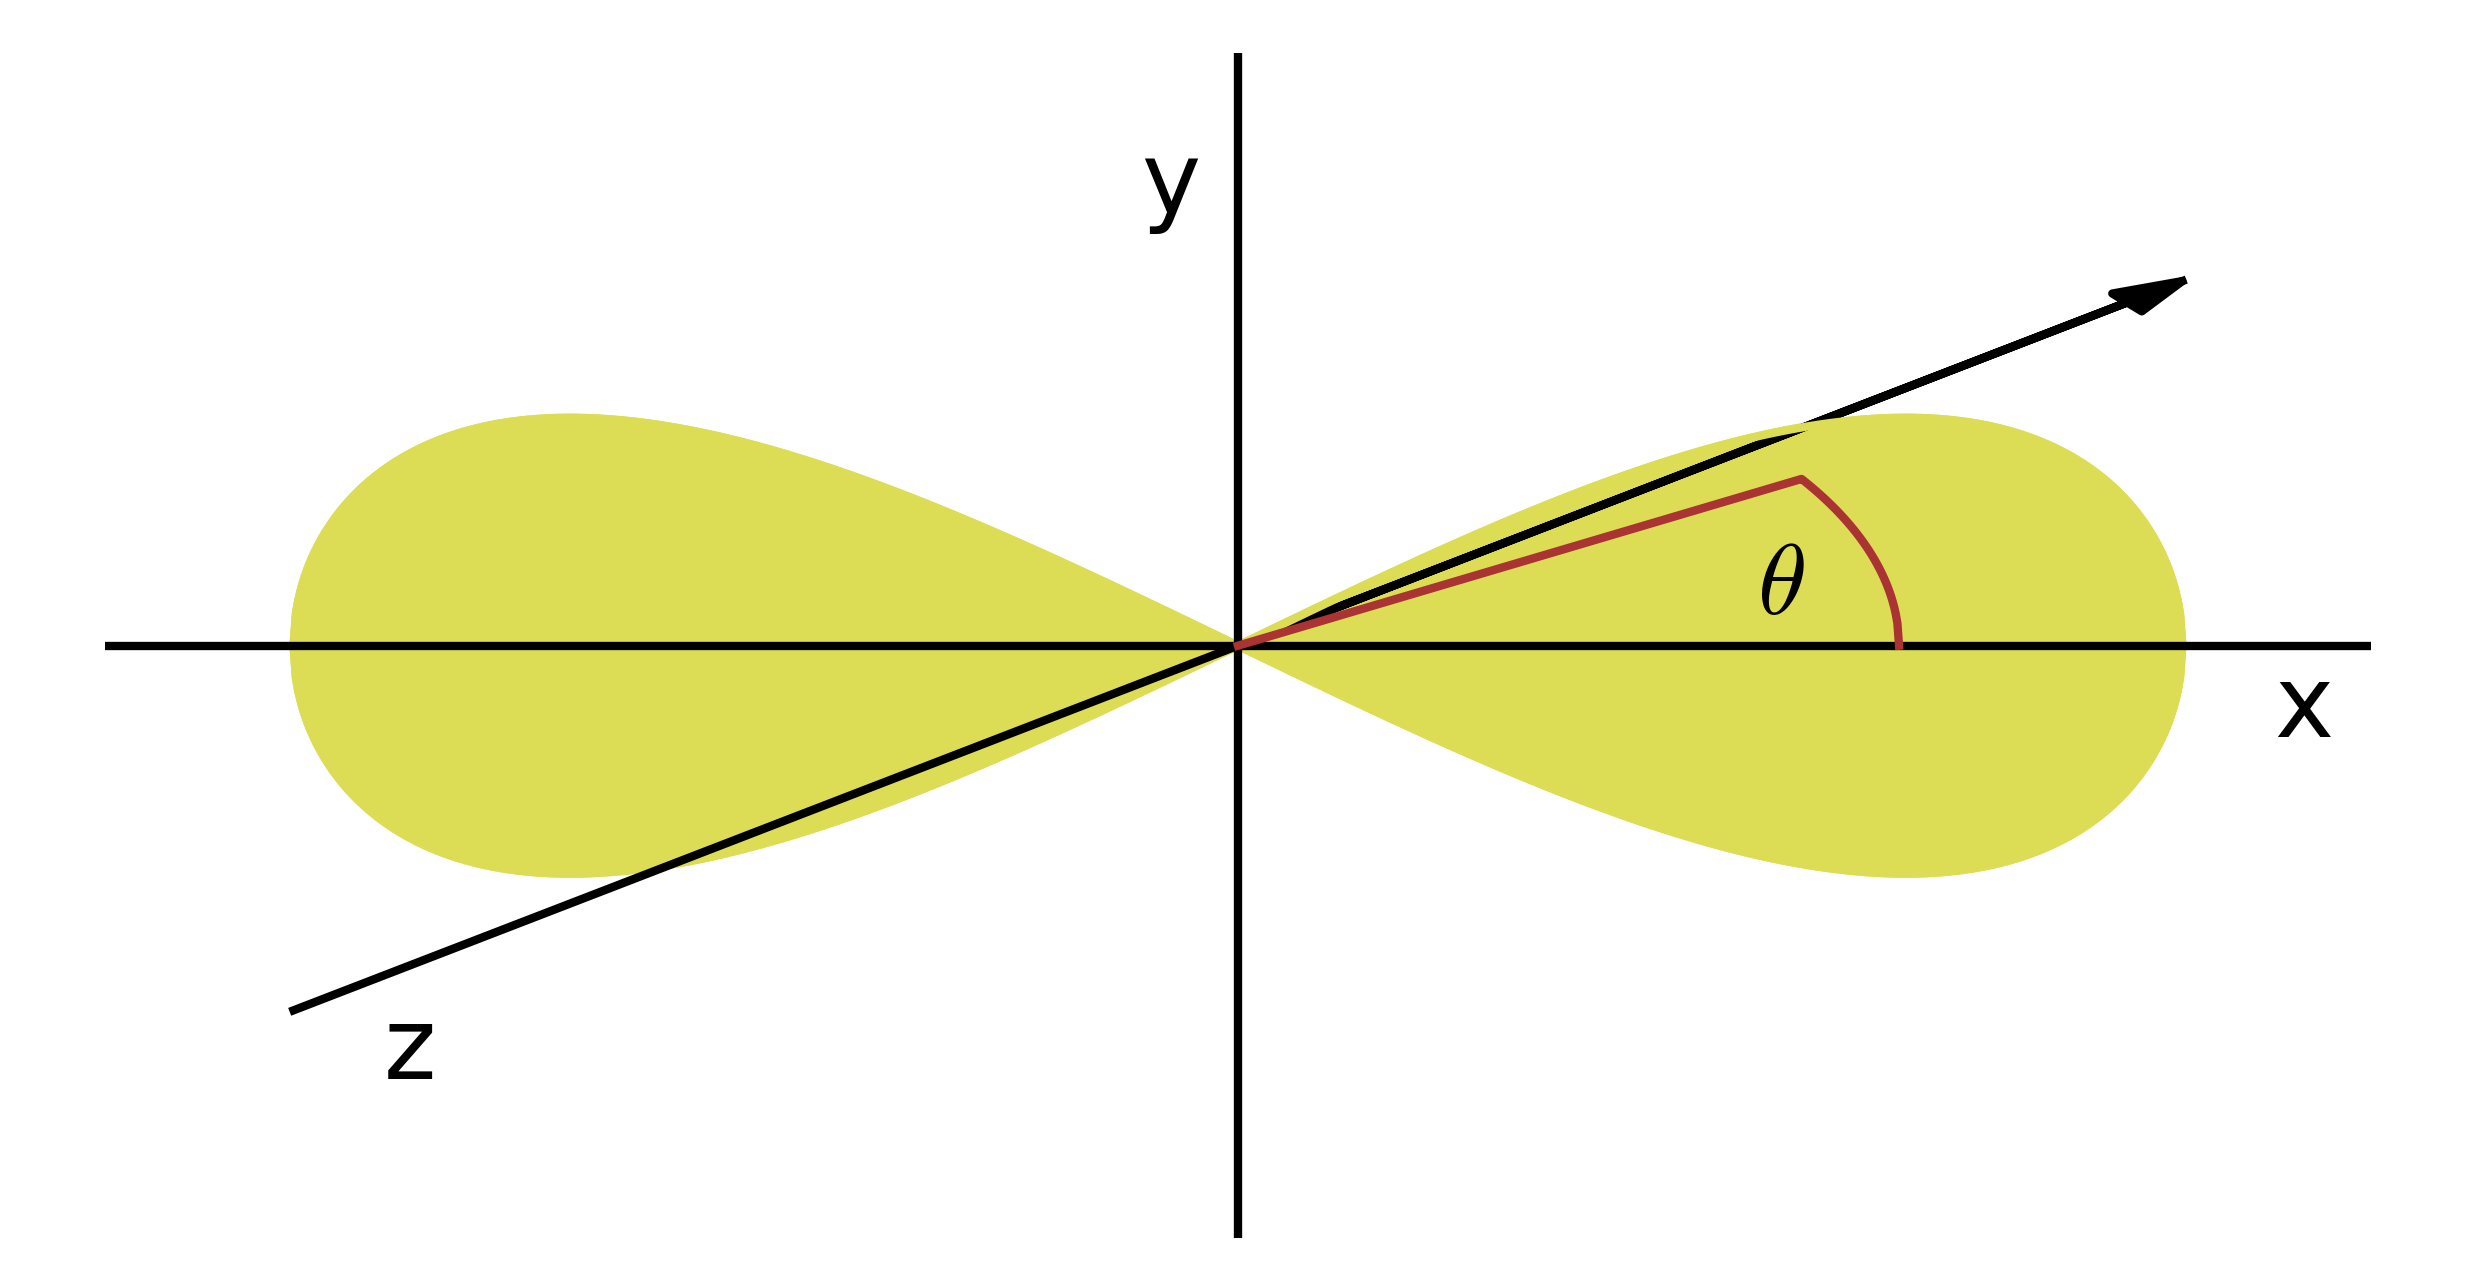
\includegraphics[width=50mm]{figs/theory/dipole}
  \end{column}
  \end{columns}

  \begin{cenpage}{110mm}

  For anisotropic systems (surfaces, non-cubic crystals, \ldots) this can
  be important:  It can be either confounding or useful!

  \vmm\vmm

  \begin{columns}
    \begin{column}{20mm}
      \wgraph{18mm}{xtals/YBCO}

     \end{column}
     \begin{column}{75mm}
       Anistropy of the {\RedEmph{crystal}} doesn't really matter
       -- anisotropy in the {\RedEmph{local structure}} does.

       \vmm

       A sorbed ion on a surface, or ion intercalated in a layered
       material, may show very strong polarization dependence.

     \end{column}
 \end{columns}

 \end{cenpage}

\vfill
\end{slide}

 
\section{Theory/Complications: Disorder Terms}

\begin{slide}{Structural Disorder and the Pair Distribution Function}


  \begin{cenpage}{120mm}

    
  An EXAFS measurement averages billions of {\BlueEmph{snapshots}} of the
  local structure:

  \onslide+<2->
  
    \begin{itemize}
    \item Each absorbed x-ray generates 1 photo-electron.
    \item the photo-electron / core-hole pair lives for about
      $10^{-15}$ s --  much faster than the timescale for thermal vibrations ($10^{-12}$ s).
    \item An EXAFS measurement samples $10^4$ (dilute fluorescence) to $10^{10}$
      absorbed x-rays for each energy point.
    \end{itemize}
  
  \vmm \onslide+<3->
  \vmm
  
  So far, we've put this in the EXAFS Equation as \hspace{2mm}
  $\chi \sim N \exp({-2k^2\sigma^2}) $
  
  \vmm \hrule \vmm \onslide+<4->
  
  \begin{columns}
  \begin{column}{50mm}
    More generally, EXAFS samples the
    
    \vmm
    {\RedEmph{Partial Pair Distribution Function}}
    
    \vmm
    
    {\RedEmph{$g(R)$}} =   probability that an
    atom is a distance $R$ away from the absorber.
    
    \vmm\vmm

    For now, we'll just note that this may need to be taken into account.
    
    
  \end{column}
  \begin{column}{70mm}
    
    \scalebox{1}{\wgraph{65mm}{errors/gnxas}}
  \end{column}
\end{columns}

\end{cenpage}

\end{slide}



 

\begin{slide}{The EXAFS Equation: Recap}


  \begin{cenpage}{120mm}

    Even with all those complications and caveats, we still use the
    {\BlueEmph{EXAFS Equation}}: \vspace{-1mm}

  \begin{center}
    \[ \chi(k) = \sum_j {\frac{{\Blue{N_j}} {\Red{f_j(k)}}
        e^{-2{\Blue{R_j}}/{\Red{\lambda(k)}}}
        e^{-2k^2{\Blue{\sigma_j^2}}}}{k{\Blue{R_j}}^2}
      {\sin[{2k{\Blue{R_j}} + {\Red{\delta_j(k)}}] }}} \]
  \end{center}

  \vmm

  where $\Red{f(k)}$ and $\Red{\delta(k)}$ are
  {\RedEmph{photo-electron scattering properties}} of the neighboring
  atom and $ \Red{\lambda(k)} $ is the photo-electron mean-free-path.

  \vmm


  \vmm
Again, if we know these properties, we can determine:
  \onslide+<2->
    \begin{description}
      \settowidth{\labelwidth}{15mm}
      \setlength{\itemindent}{15mm}
      \setlength{\leftmargin}{15mm}
    \item[$R$] distance to neighboring atom.
    \item[$N$] coordination number of neighboring atom.
    \item[$\sigma^2$] mean-square disorder of neighbor distance \par
      \hspace{13.5mm} (or
      more complicated disorder terms).
    \end{description}

  \vmm
  \onslide+<3>
  ${\Red{f(k)}}$ and ${\Red{\delta(k)}}$ depend on atomic number
  {\BlueEmph{Z}} of the scattering atom, so we can also determine the
  species of the neighboring atom.

\end{cenpage}

\end{slide}


\begin{slide}{EXAFS Theory:  Conclusions}
  
  \begin{cenpage}{110mm}
    We have an EXAFS Equation that we can use to model EXAFS data.

  \begin{center}
    \[ \chi(k) = \sum_j {\frac{{\Blue{N_j}} {\Red{f_j(k)}}
        e^{-2{\Blue{R_j}}/{\Red{\lambda(k)}}}
        e^{-2k^2{\Blue{\sigma_j^2}}}}{k{\Blue{R_j}}^2}
      {\sin[{2k{\Blue{R_j}} + {\Red{\delta_j(k)}}] }}} \]
  \end{center}

  \vmm
  In later videos and demos we'll show how to use this for
  analyzing EXAFS data.

  

  \vmm\vmm \hrule \vmm
  
  More information on X-rays and X-ray Absorption Spectroscopy:

  \begin{itemize}
  \item[] {\Blue{https://xafs.xrayabsorption.org/}}
  \item[] {\BlueEmph{Fundamentals of XAFS}} M. Newville, Reviews in  Mineralogy \& Geochemistry {\bf{78}}, 2014.
  \item[] {\BlueEmph{Introduction to XAFS}} G. Bunker, Cambridge Univ  Press,  2010.
  \item[] {\BlueEmph{XAFS for Everyone}} S. Calvin, CRC Press, 2013.
  \item[]  {\BlueEmph{Elements of Modern X-ray Physics}}  J.~Als-Nielsen
    \& D.~McMorrow,  John Wiley \& Sons. 2001
    
  \end{itemize}

\end{cenpage}


 \vfill
\end{slide}
 


\end{document}


